\chapter{Event Selection}
\label{chap:Evt}

Events are required to contain exactly two \emph{tight} leptons and one \emph{tight} tau, described in \autoref{chap:Obj}. A combination of single- and di-lepton \ac{HLT} triggers are used to select data as well as simulated events. The sum of the electric charges of all three leptons is required to be 1 or -1, which guarantees at least one \ac{OSDF} pair in every selected event. Depending on the flavors and the charge assignments of the two leptons, events are further categorized into 6 different channels, which are described in \autoref{sec:Cat}. \acp{SR} require additional selection criteria to achieve an optimal signal-to-background ratio, which is discussed in \autoref{sec:SRInclusive}. Control regions of the \ac{DY} background near the Z resonance are also defined to study the accuracy of the \ac{MC} modeling, which is described in \autoref{sec:DY_CR}. 
%%%%%%%%%%%%%%%%%%%%%%%%%%%%%%%%%%%%%%%%%%%%%%%%%%
%%%%%%%%%%%%%%%%%%%%%%%%%%%%%%%%%%%%%%%%%%%%%%%%%%
\section{Event Categorization}
\label{sec:Cat}

The two \emph{tight} leptons can come with any flavor- or charge-compositions, which contain 6 possibilities: i) \ac{OS}-ee, ii) \ac{OS}-e$\upmu$, iii) \ac{OS}-$\upmu\upmu$, iv) \ac{SS}-ee, v) \ac{SS}-e$\upmu$, and vi) \ac{SS}-$\upmu\upmu$. These subsets of the selected events are referred to as ``channels'' in this analysis. The \ac{OS}-e$\upmu$ and \ac{SS}-e$\upmu$ channels are further subdivided into ``subchannels'' as more than one charged-lepton flavor mixing mode is possible in these channels. For example, due to the requirement on the sum of electric charges, the sign of the selected tau must be different from the signs of the electron and muon in the \ac{SS}-e$\upmu$ channel. This means both the e$\uptau$ and $\upmu\uptau$ flavor mixing modes are possible under such a scenario. This two-fold ambiguity is resolved by using the existing strategy described in \autoref{sec:Kin}: two \ac{SM} quark candidates are reconstructed by combining the \ac{MET}, the jet with the highest \DeepJ score, and two leptons in question. The lepton that gives a top quark mass that is closer to 172.5 GeV is assigned as the standalone lepton while the other lepton is assigned as the LFV lepton that contributes to the flavor mixing. There is only one subchannel for each of the other four channels as there is no ambiguity on how to assign the mixing mode to events residing in these four channels. A total of 9 subchannels are defined, which is illustrated in Figure~\ref{fig:EvtCat}. 

As is shown in \ref{fig:SigGen}, the invariant mass of the LFV-dilepton pair of any mixing mode, denoted by m($\ell\ell^{\prime}$), has a sharp end point at around 150 GeV for top quark decay signals. Such a pattern does not exist in the top quark production signals. Therefore, each subchannel is further subdivided into two search bins to create regions enriched in different signal modes using a threshold of 150 GeV on m($\ell\ell^{\prime}$), which leads to a total of 18 search bins. The strategy of creating high (low) mass \acp{SR} to target top quark production (decay) signals are taken from the previous analysis.

\begin{figure}[tbh!]
 \begin{center}
 \begin{tabular}{c}
 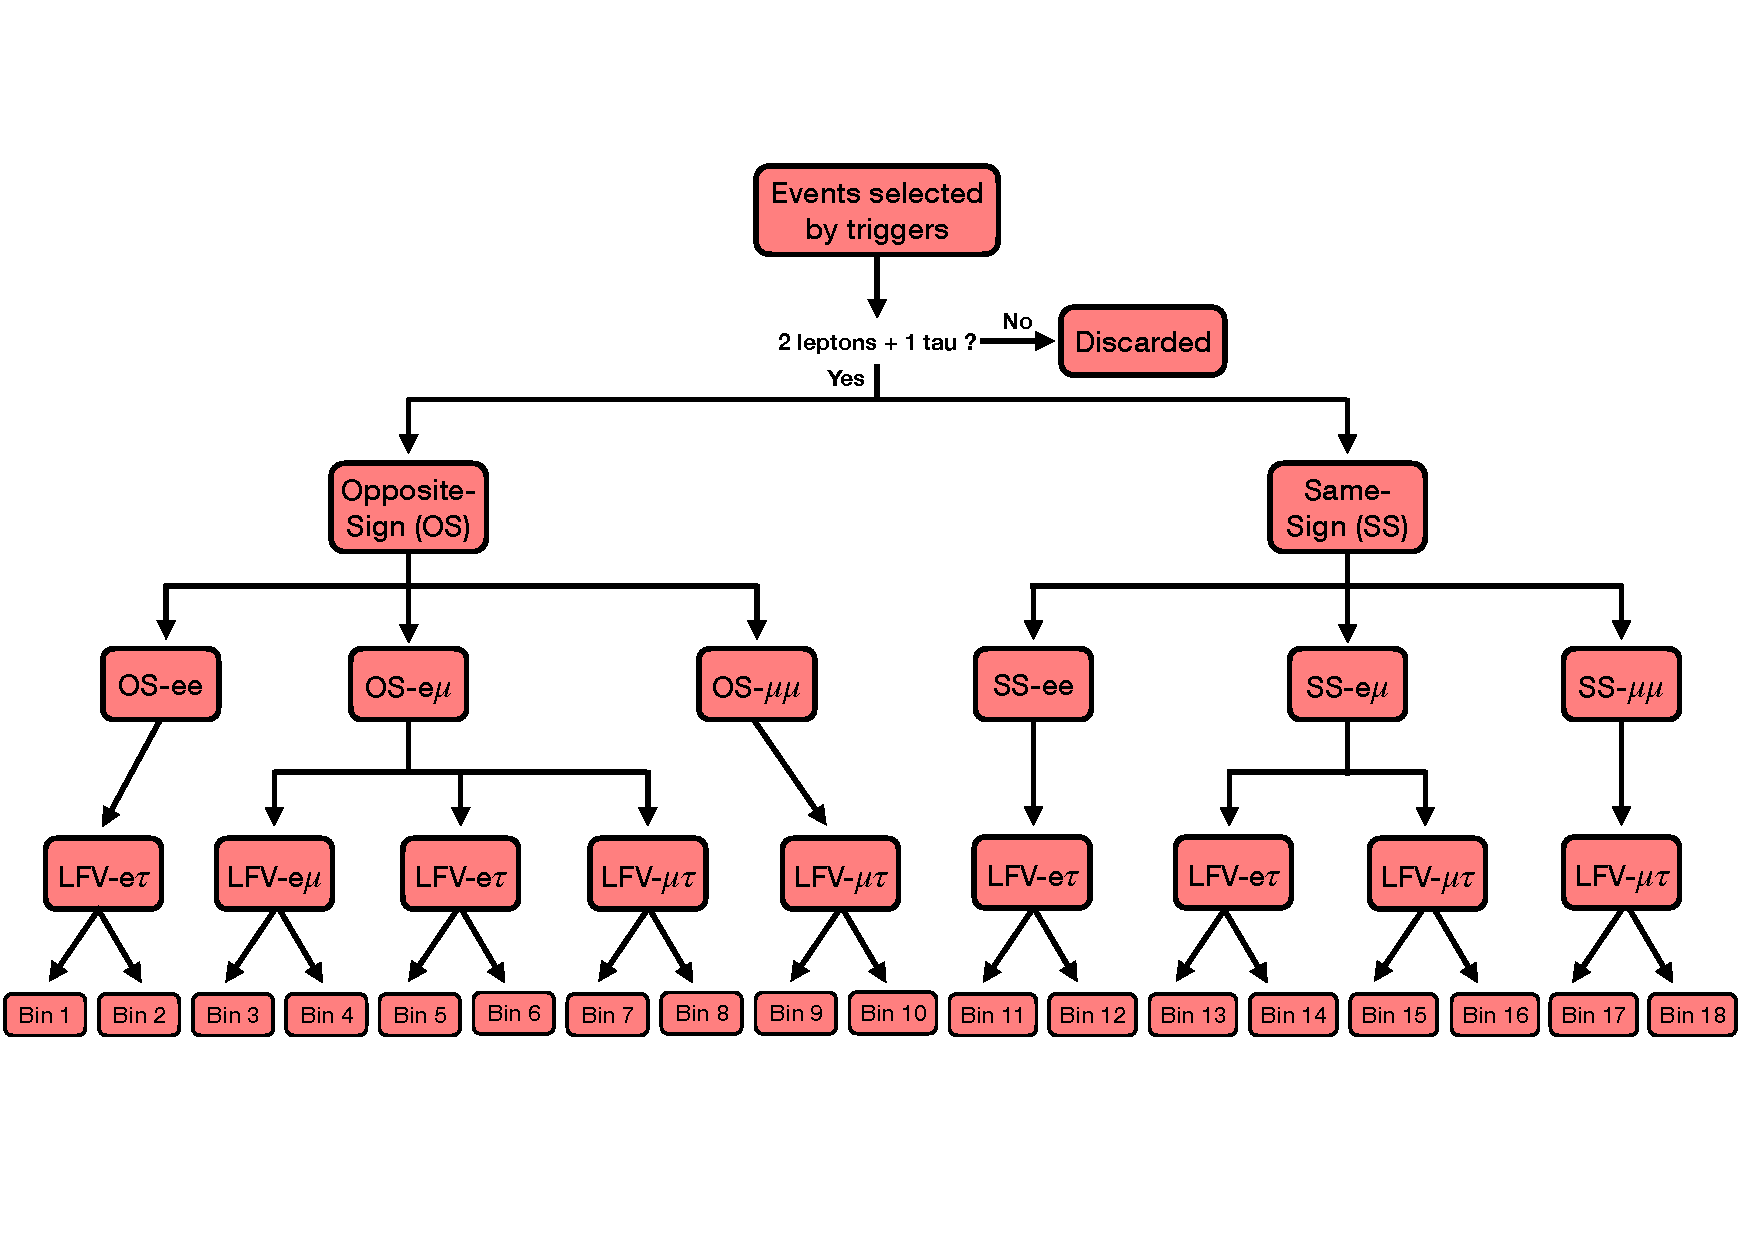
\includegraphics[width=\textwidth]{figures/Part4/Evt/SRFlowChart}
 \end{tabular}
 \caption{Illustration of event categorization scheme used by this analysis. The second to the last row shows 9 exclusive subchannels, where a specific charged-lepton flavor mixing mode is assigned. The odd (even) bins shown in the last row correspond to search bins with the requirement of m($\ell\ell^{\prime}$) $<(>)$ 150 GeV.}
 \label{fig:EvtCat}
 \end{center}
 \end{figure}
 
The performance of this categorization scheme is evaluated by using simulated signal events that contain all three flavor mixing modes. An incorrect assignment occurs when a signal event is generated in one flavor mixing mode but is categorized into another flavor mixing mode. The rate of occurrences of an incorrect assignment is largely under control, as is shown in Figure~\ref{fig:SRbin}. Further improvement is possible with the assistance of more sophisticated algorithms, such as \acp{NN}. 
 
 \begin{figure}[tbh!]
 \begin{center}
 \begin{tabular}{c}
 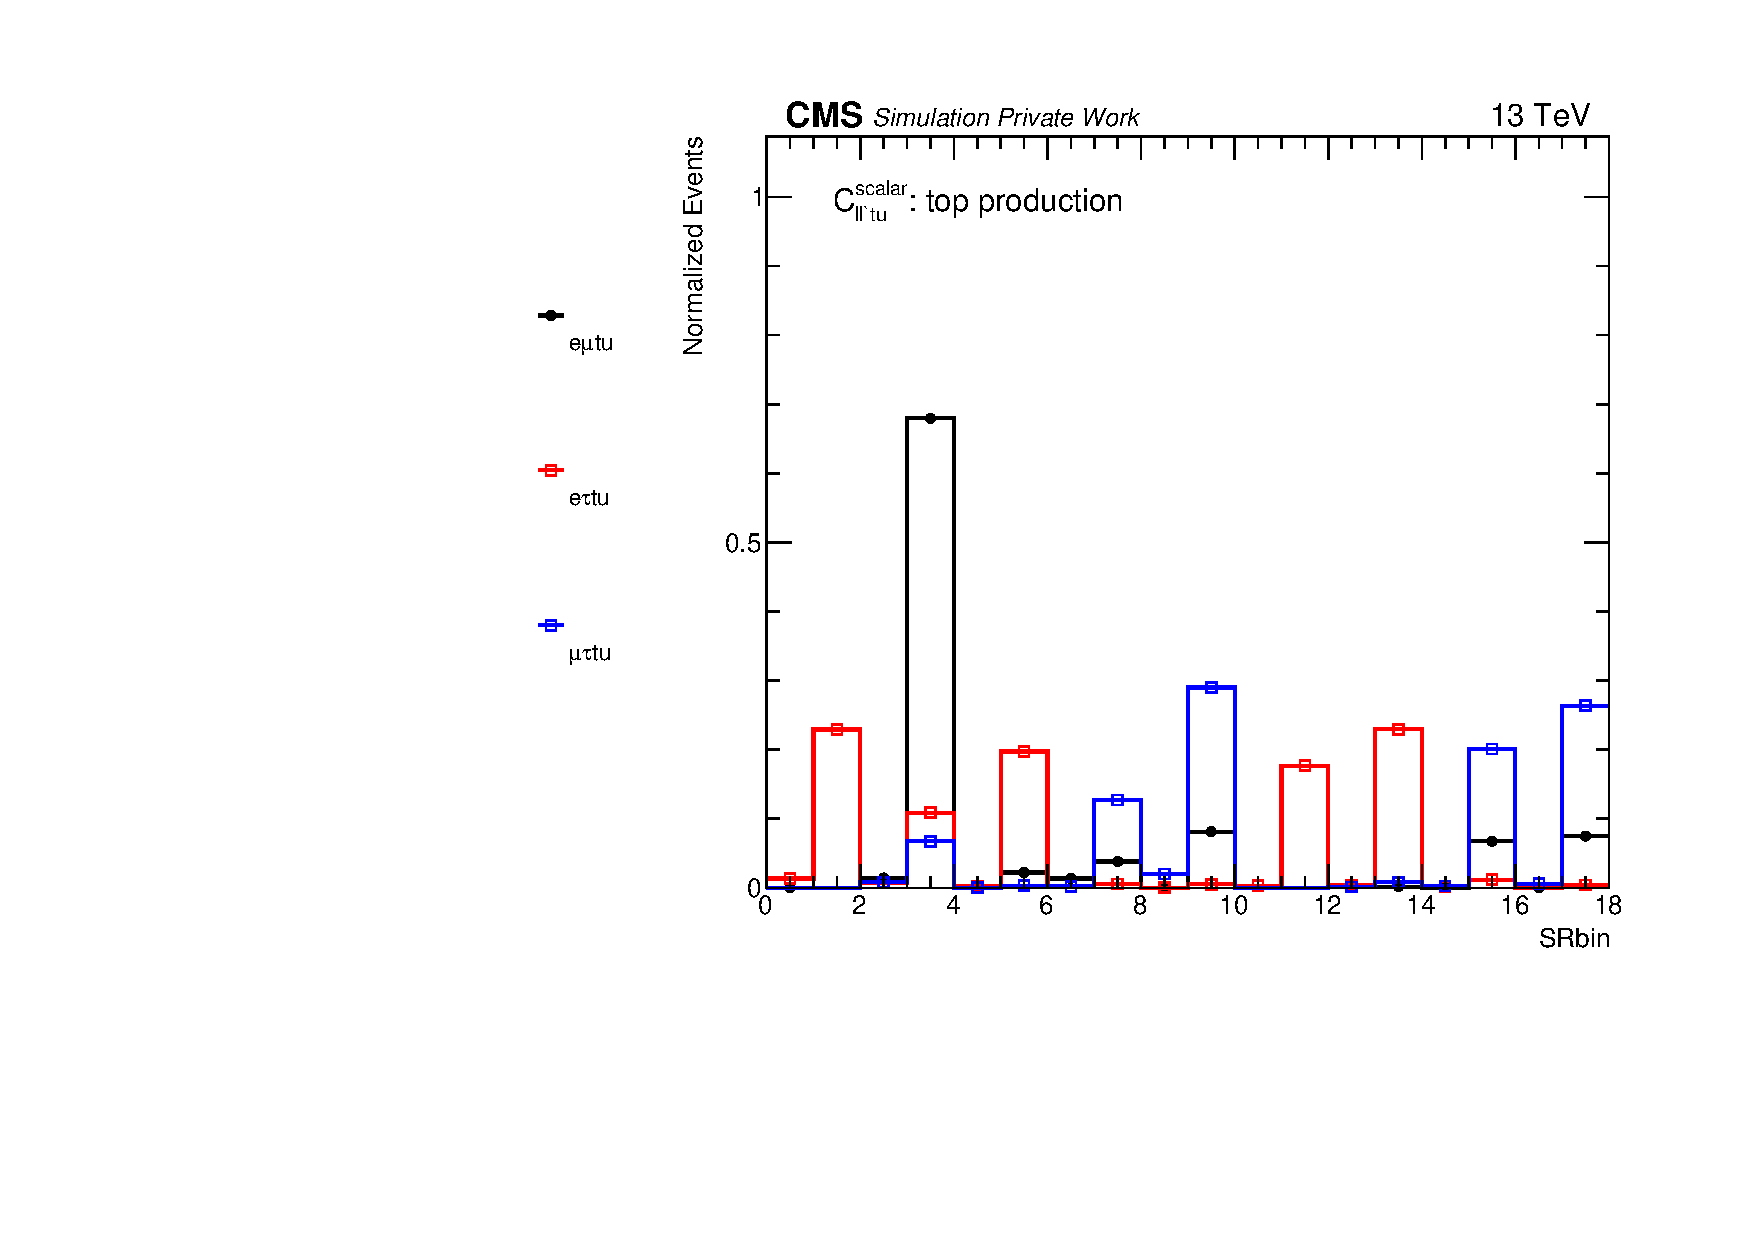
\includegraphics[width=0.9\textwidth]{figures/Part4/Evt/SRbin}
 \end{tabular}
 \caption{Normalized distribution of search bins assigned by the categorization scheme. Signal events generated in e$\upmu$, e$\uptau$, and $\upmu\uptau$ modes are shown in black, red, and blue lines respectively. The ordering of the search bins is the same as the one shown in \ref{fig:EvtCat}. }
 \label{fig:SRbin}
 \end{center}
 \end{figure}
%%%%%%%%%%%%%%%%%%%%%%%%%%%%%%%%%%%%%%%%%%%%%%%%%%
%%%%%%%%%%%%%%%%%%%%%%%%%%%%%%%%%%%%%%%%%%%%%%%%%%

\section{Signal Region}
\label{sec:SRInclusive}

To further improve the sensitivity of this analysis, additional selection criteria are used to create \acp{SR}. More specifically, events are required to contain at least one jet and exactly one b-tagged jet. A minimum \ac{MET} of 20 GeV is required to account for the presence of neutrinos due to the leptomically decaying top quark. Furthermore, events that contain an \ac{OSSF} lepton pair with an invariant mass between 58 and 108 GeV are removed to suppress the \ac{DY} background. A summary of expected signal and background events that enter \acp{SR} is shown in Figure~\ref{fig:Summary}.

\begin{figure}[tbh!]
 \begin{center}
 \begin{tabular}{c}
 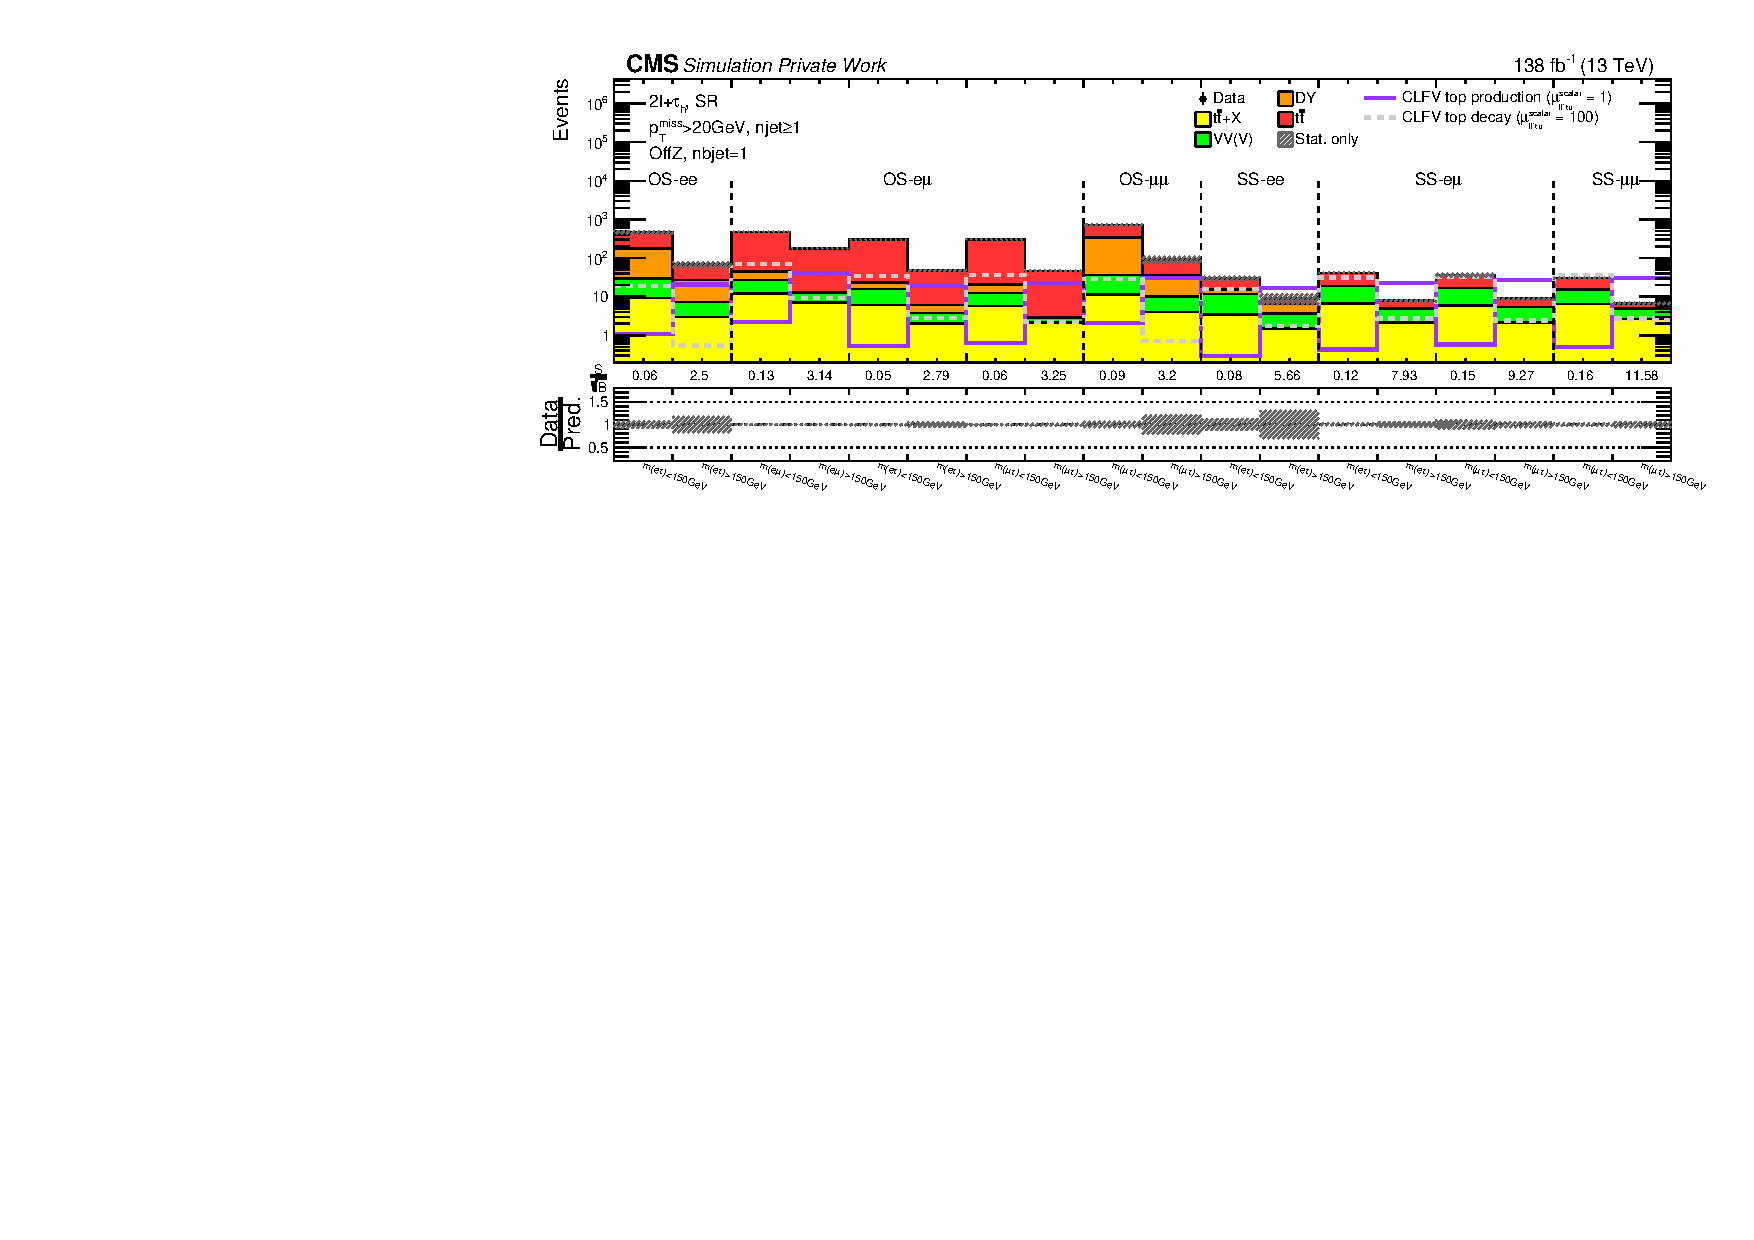
\includegraphics[width=\textwidth]{figures/Part4/Evt/Summary_llOffZMetg20B1}
 \end{tabular}
 \caption{Summary of expected signal and background events in \acp{SR}. Signal events generated in different flavor mixing modes are not combined. The original signal strength ($\mu_{\ell\ell^{\prime}\textsf{tu}}^{\textsf{scalar}}$ = 1), corresponding to $\textsf{C}_{\ell\ell^{\prime}\textsf{tu}}^{\textsf{scalar}}/\Lam^2~=~1~\TeV^{\textsf{-2}}$, is used to normalize the cross-section of top quark production signals. The cross-section of top quark decay signals is scaled up by a factor of 100 for improved visualization. Only statistical uncertainties for the background predictions are included in the hatched bands. The ordering of the search bins is the same as the one shown in \ref{fig:EvtCat}. For each search bin, the number of total signal events divided by the square root of the number of total background events is calculated and shown in the gap between the upper and lower panels.}
 \label{fig:Summary}
 \end{center}
 \end{figure}
 
Representative distributions of m($\ell\ell^{\prime}$) and $\mathrm{\Delta}R$ at reconstruction level are shown in Figure~\ref{fig:LFVmass}.
 
 \begin{figure}[tbh!]
 \begin{center}
 \begin{tabular}{ccc}
 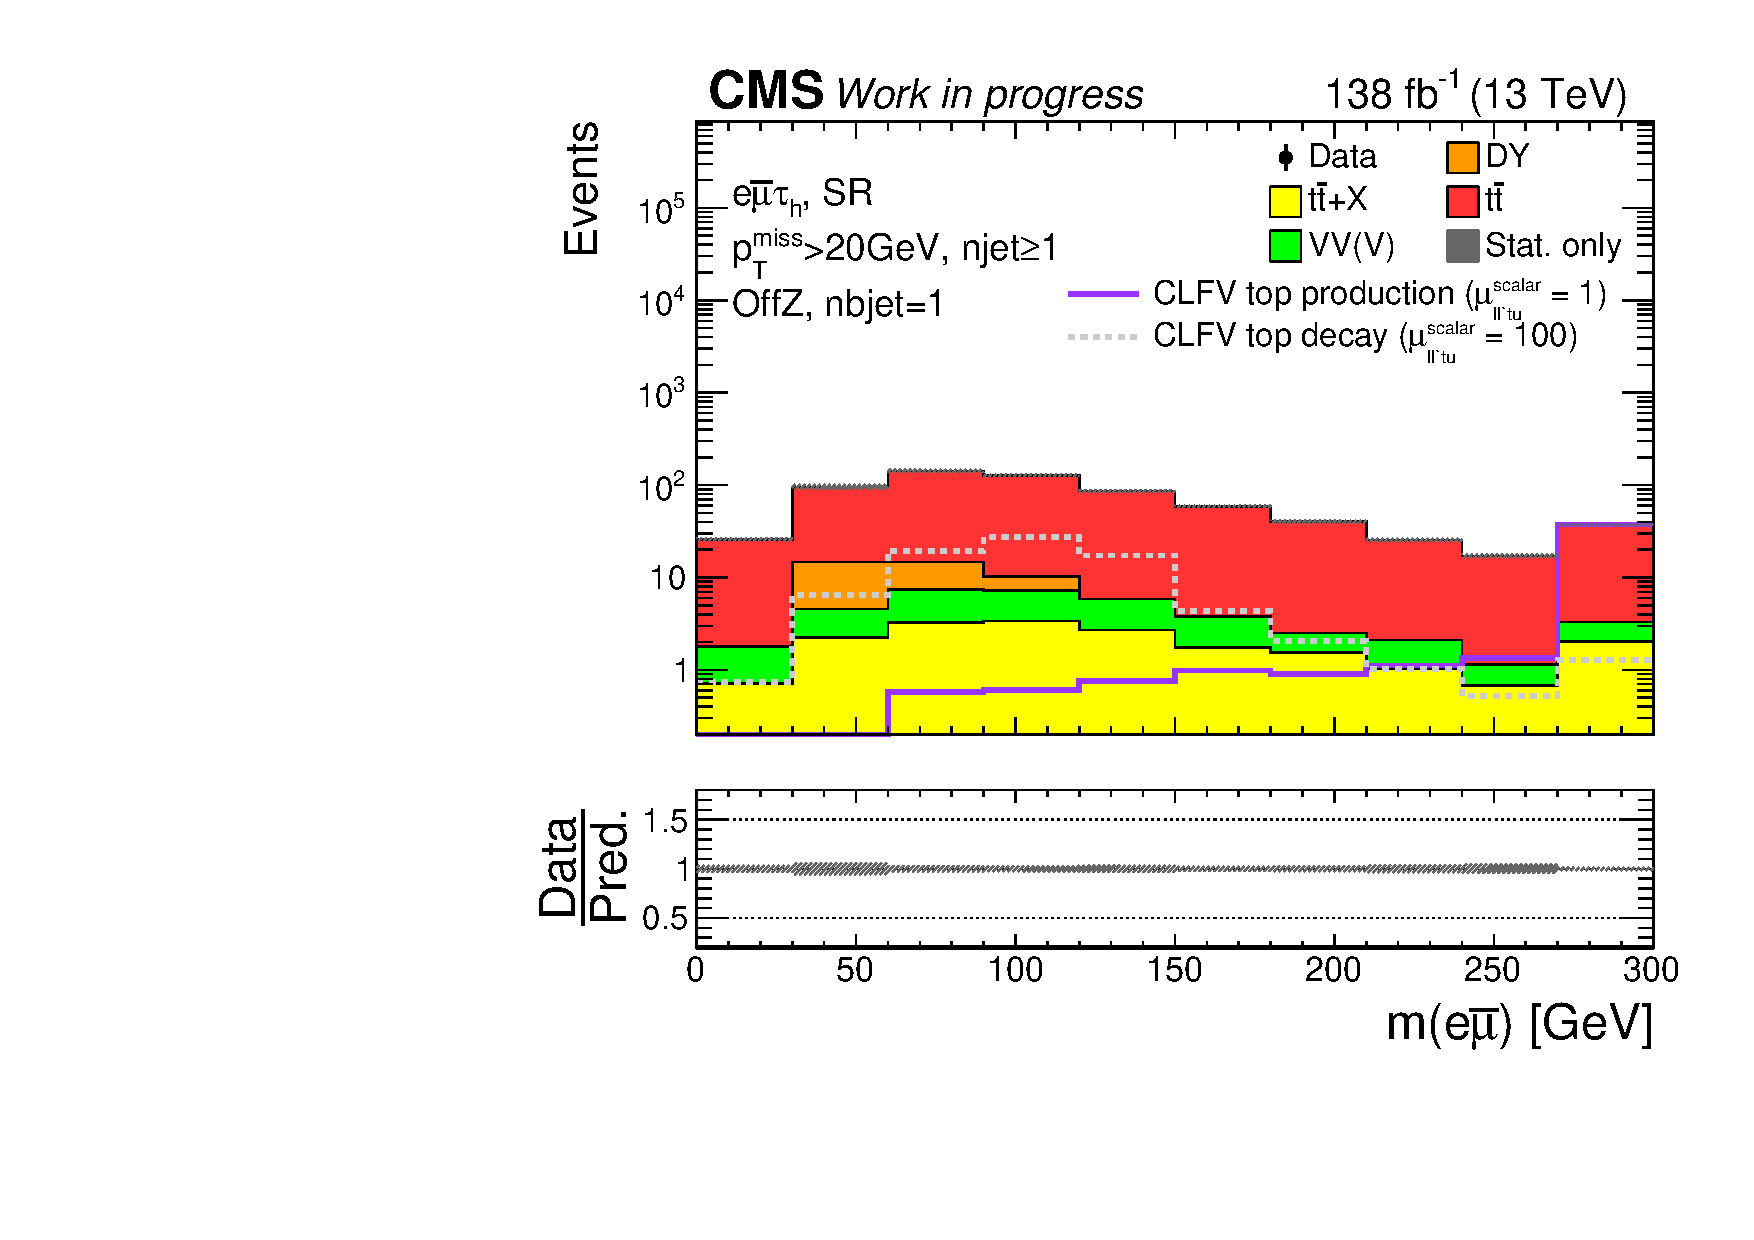
\includegraphics[width=0.33\textwidth]{figures/Part4/Evt/LFVemuM}&
 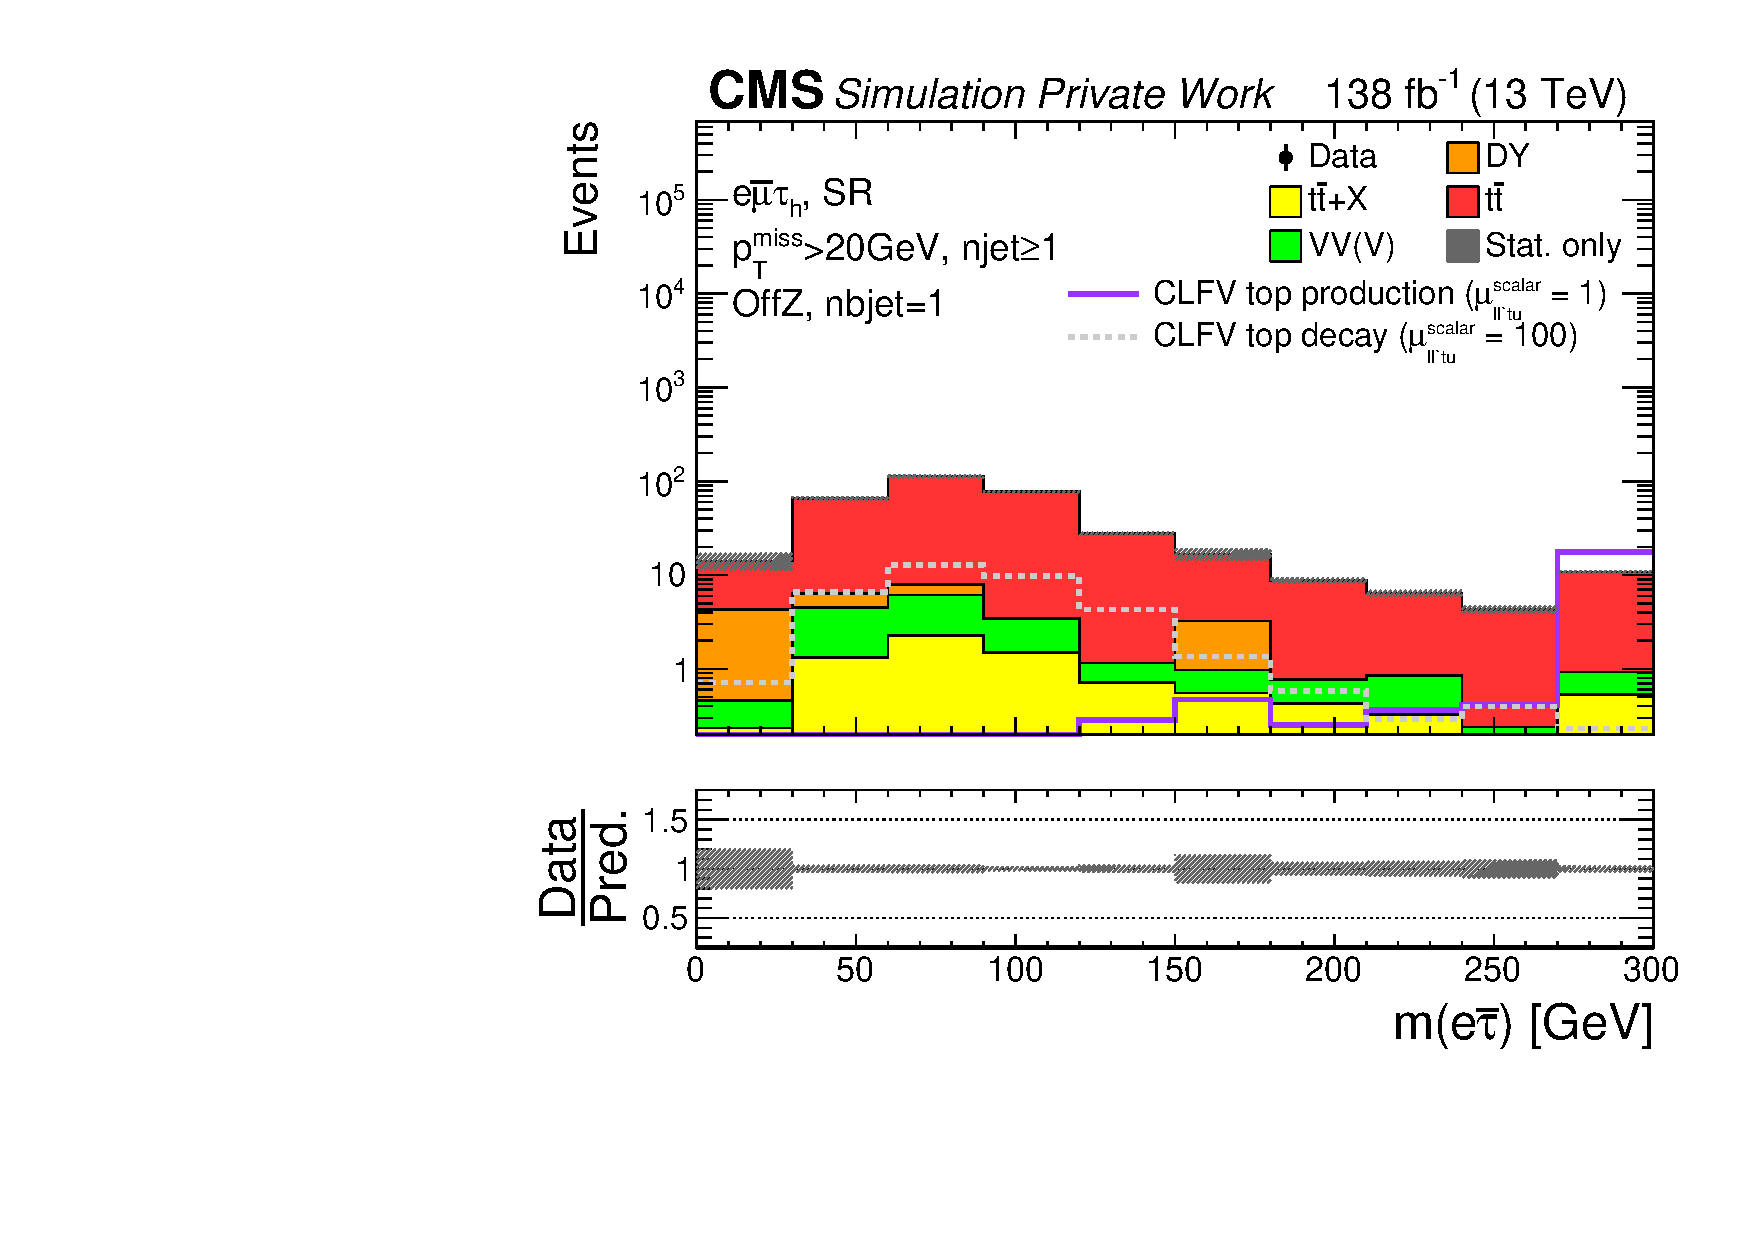
\includegraphics[width=0.33\textwidth]{figures/Part4/Evt/LFVetaM}&
 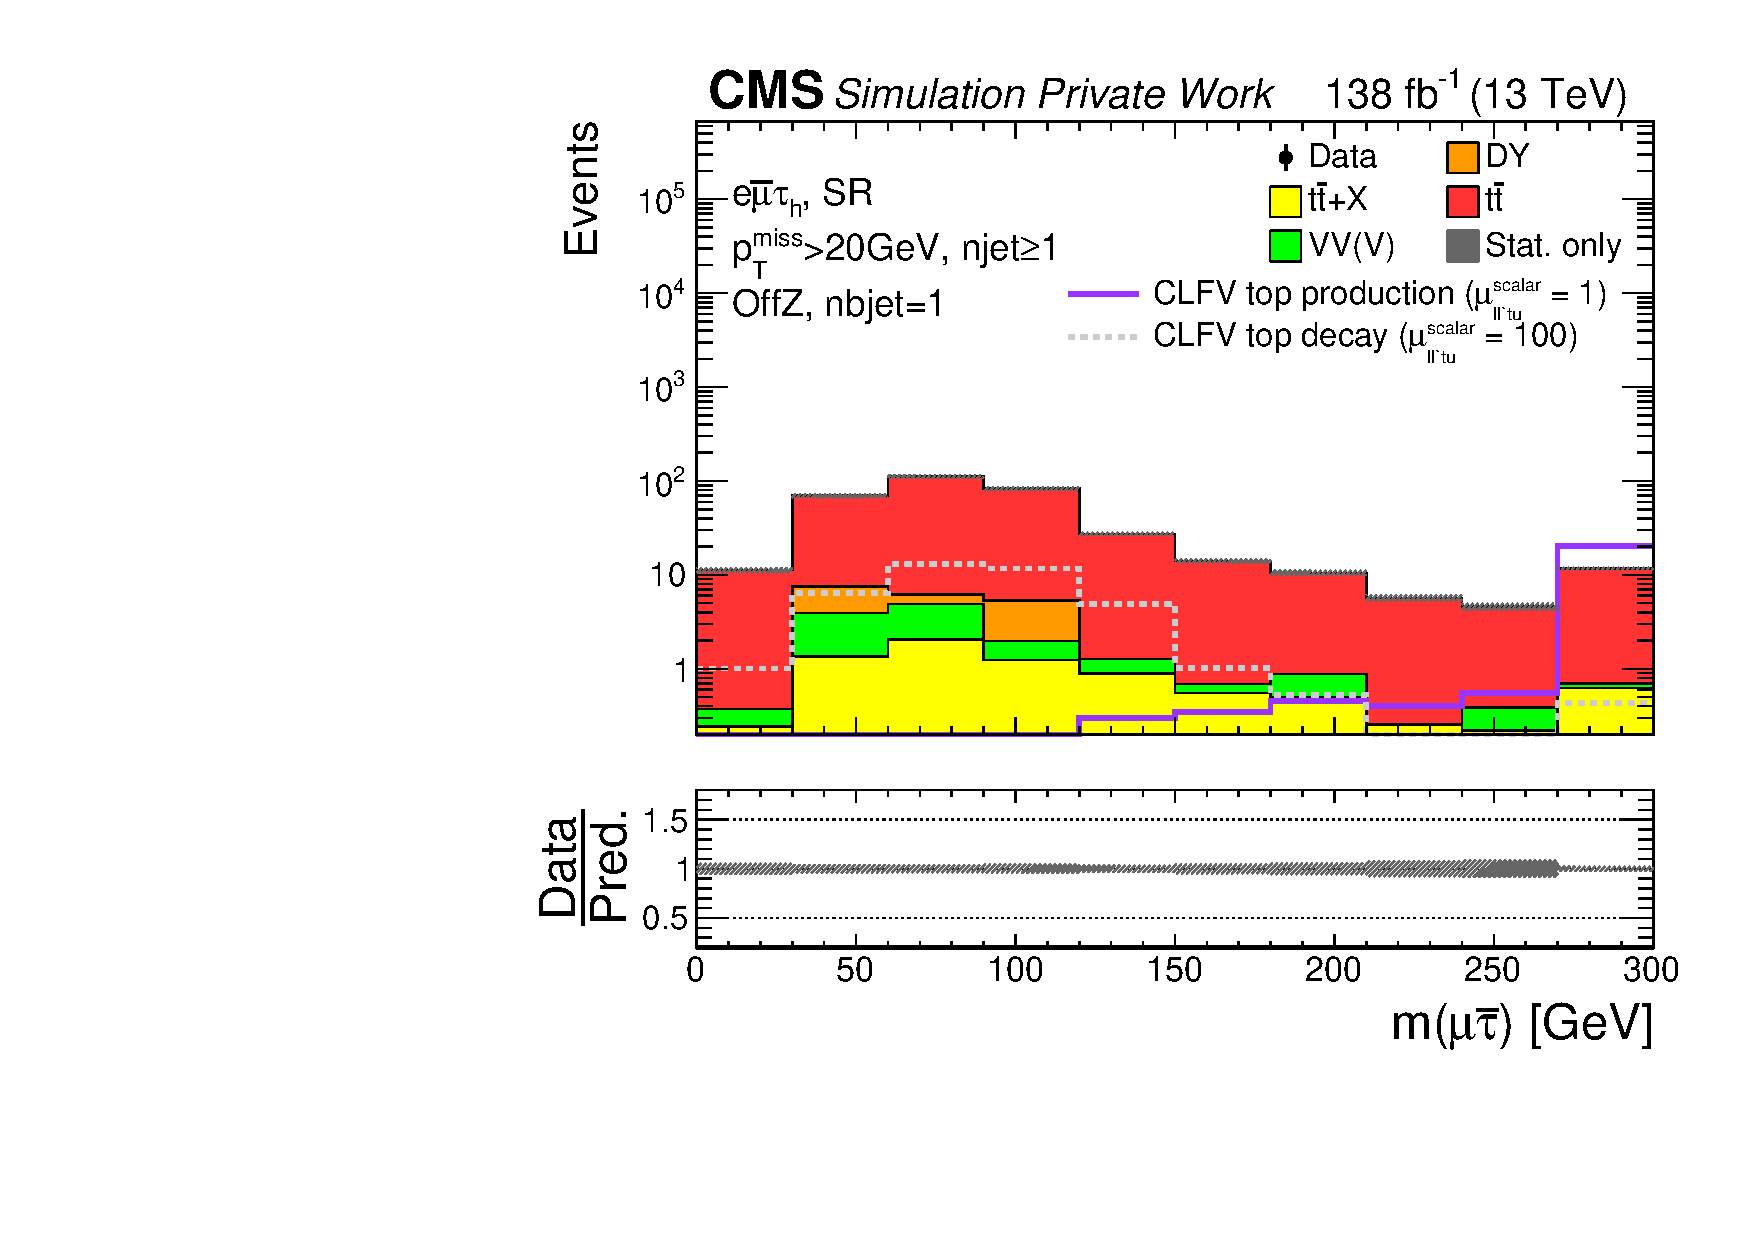
\includegraphics[width=0.33\textwidth]{figures/Part4/Evt/LFVmutaM}\\
 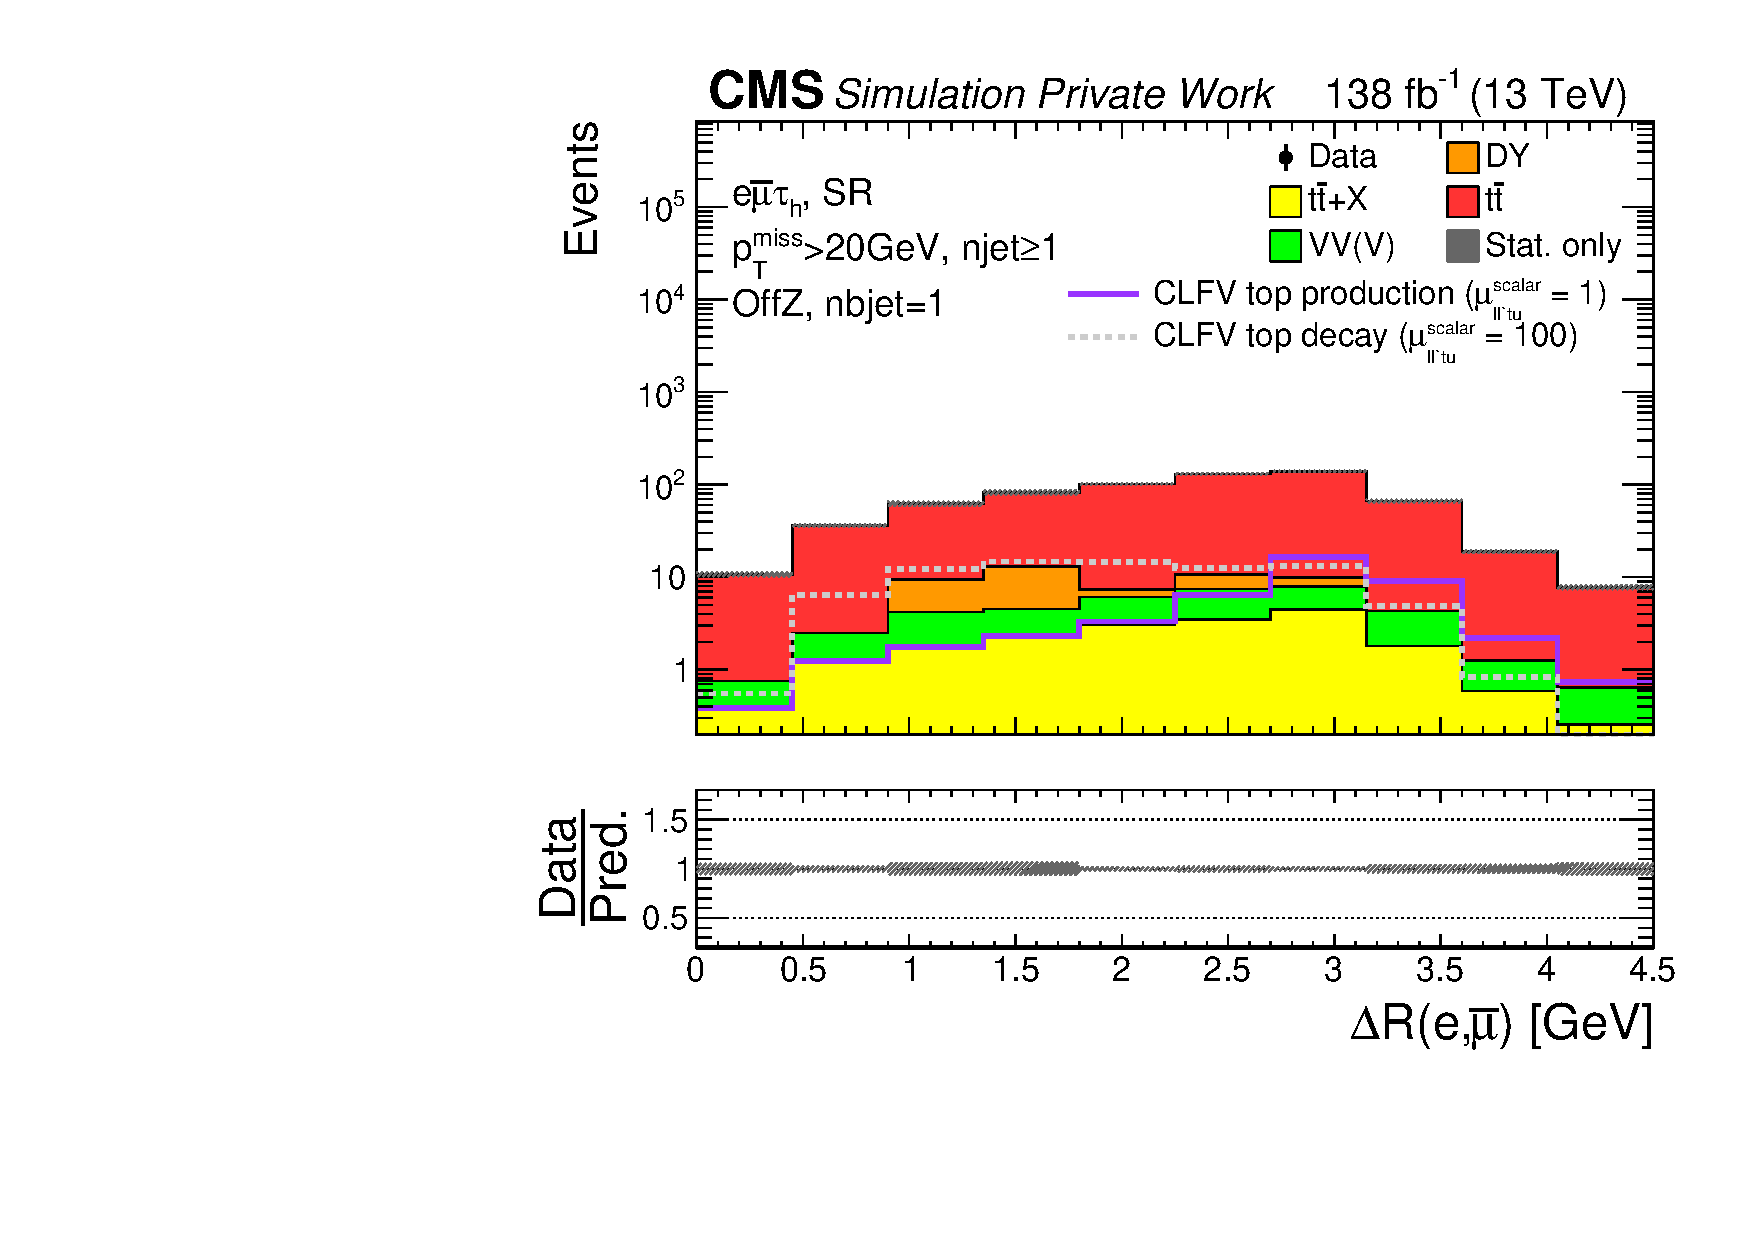
\includegraphics[width=0.33\textwidth]{figures/Part4/Evt/LFVemuDr}&
 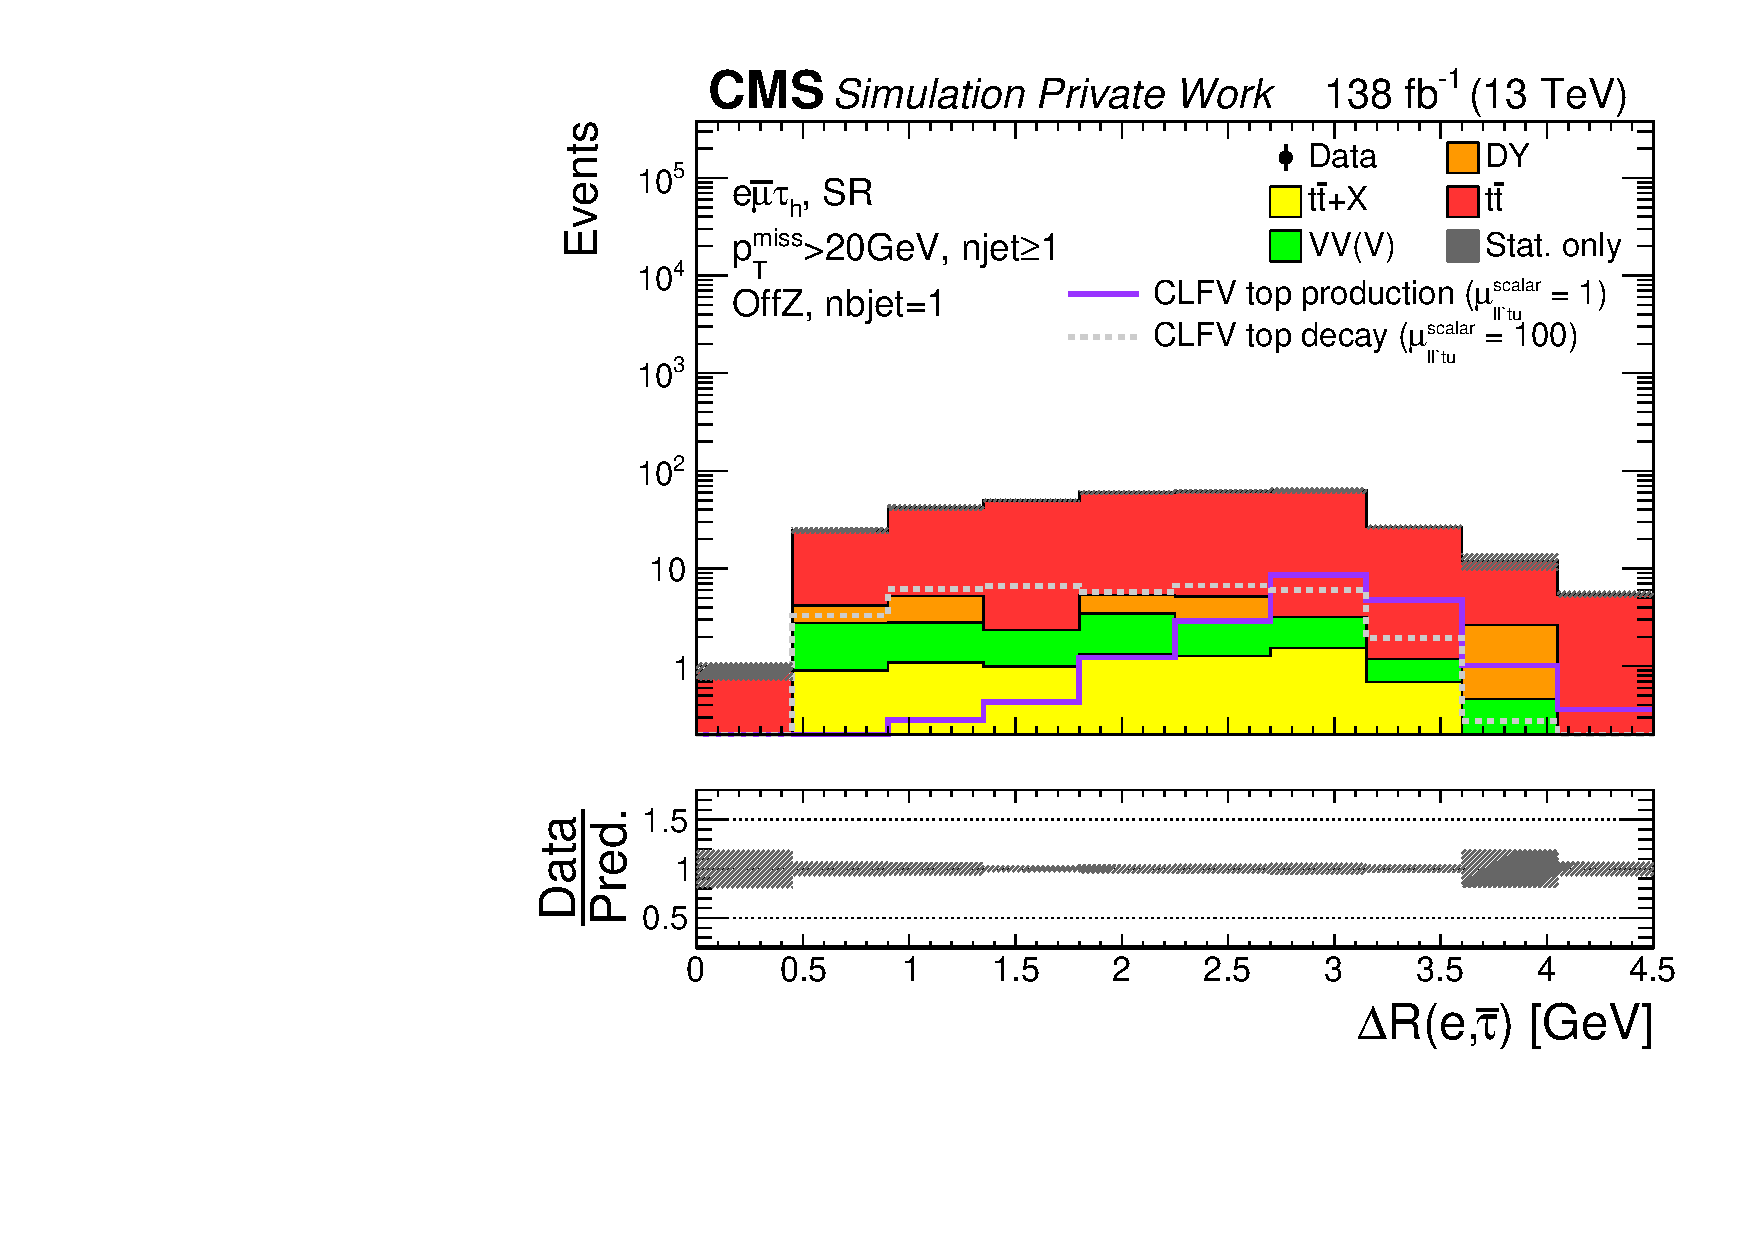
\includegraphics[width=0.33\textwidth]{figures/Part4/Evt/LFVetaDr}&
 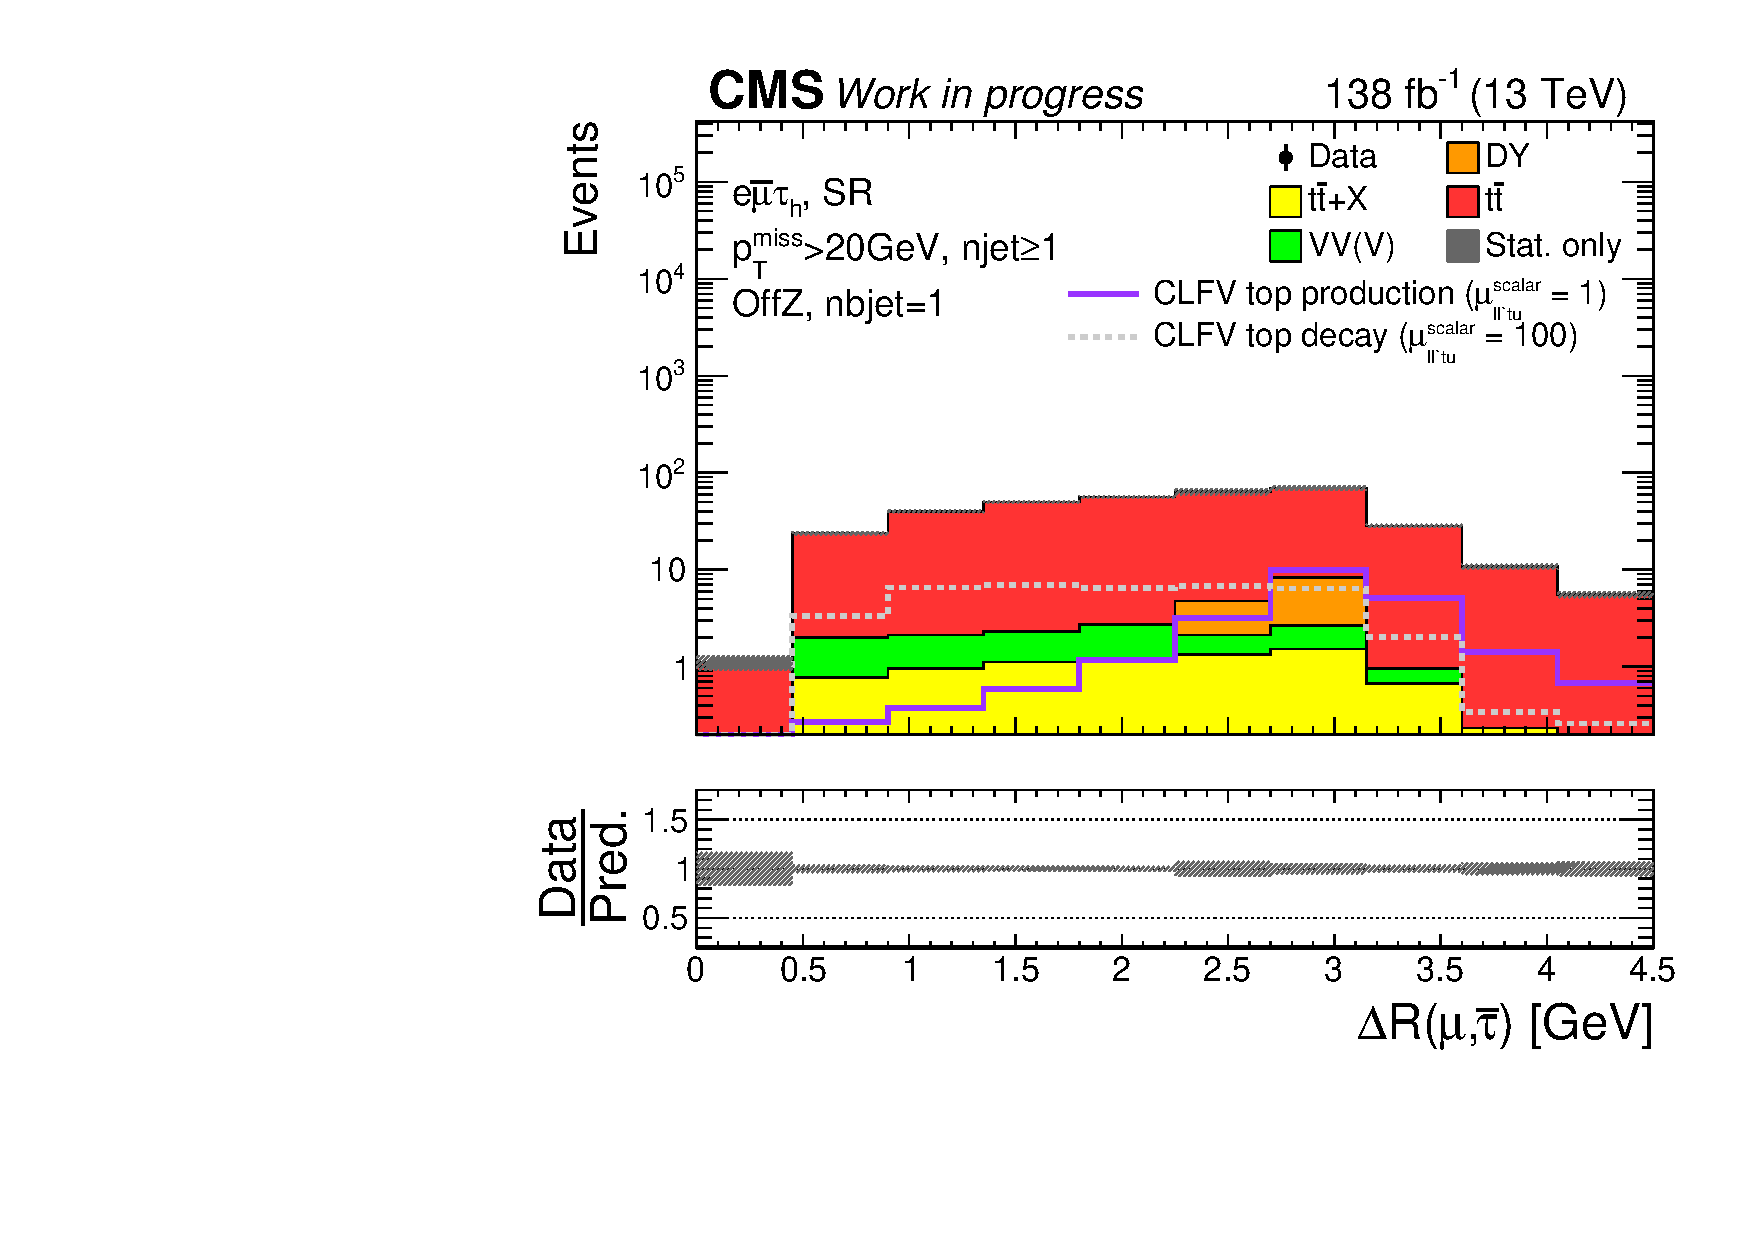
\includegraphics[width=0.33\textwidth]{figures/Part4/Evt/LFVmutaDr}\\
 \end{tabular}
 \caption{Distributions of the LFV-dilepton mass (top row) and opening angle between the two LFV leptons (bottom row) in the \acp{SR} in the \ac{OS}-e$\upmu$ channel. Events categorized into the LFV e$\upmu$, LFV e$\uptau$, and LFV $\upmu\uptau$ subchannels are shown in the left column, middle column, and right column, respectively. The hatched bands only include statistical uncertainties for the background predictions. The last bin of all histograms includes the overflow events.}
 \label{fig:LFVmass}
 \end{center}
 \end{figure}
%%%%%%%%%%%%%%%%%%%%%%%%%%%%%%%%%%%%%%%%%%%%%%%%%%
%%%%%%%%%%%%%%%%%%%%%%%%%%%%%%%%%%%%%%%%%%%%%%%%%%

\section{Drell-Yan Control Region}
\label{sec:DY_CR}

The Z mass veto used to define \acp{SR} is reversed to create regions enriched in \ac{DY} events. Distributions of the \ac{OSSF} lepton mass and jet multiplicity in the \ac{DY} control regions are shown in Figure~\ref{fig:DY_CR}.

 \begin{figure}[tbh!]
 \begin{center}
 \begin{tabular}{cc}
 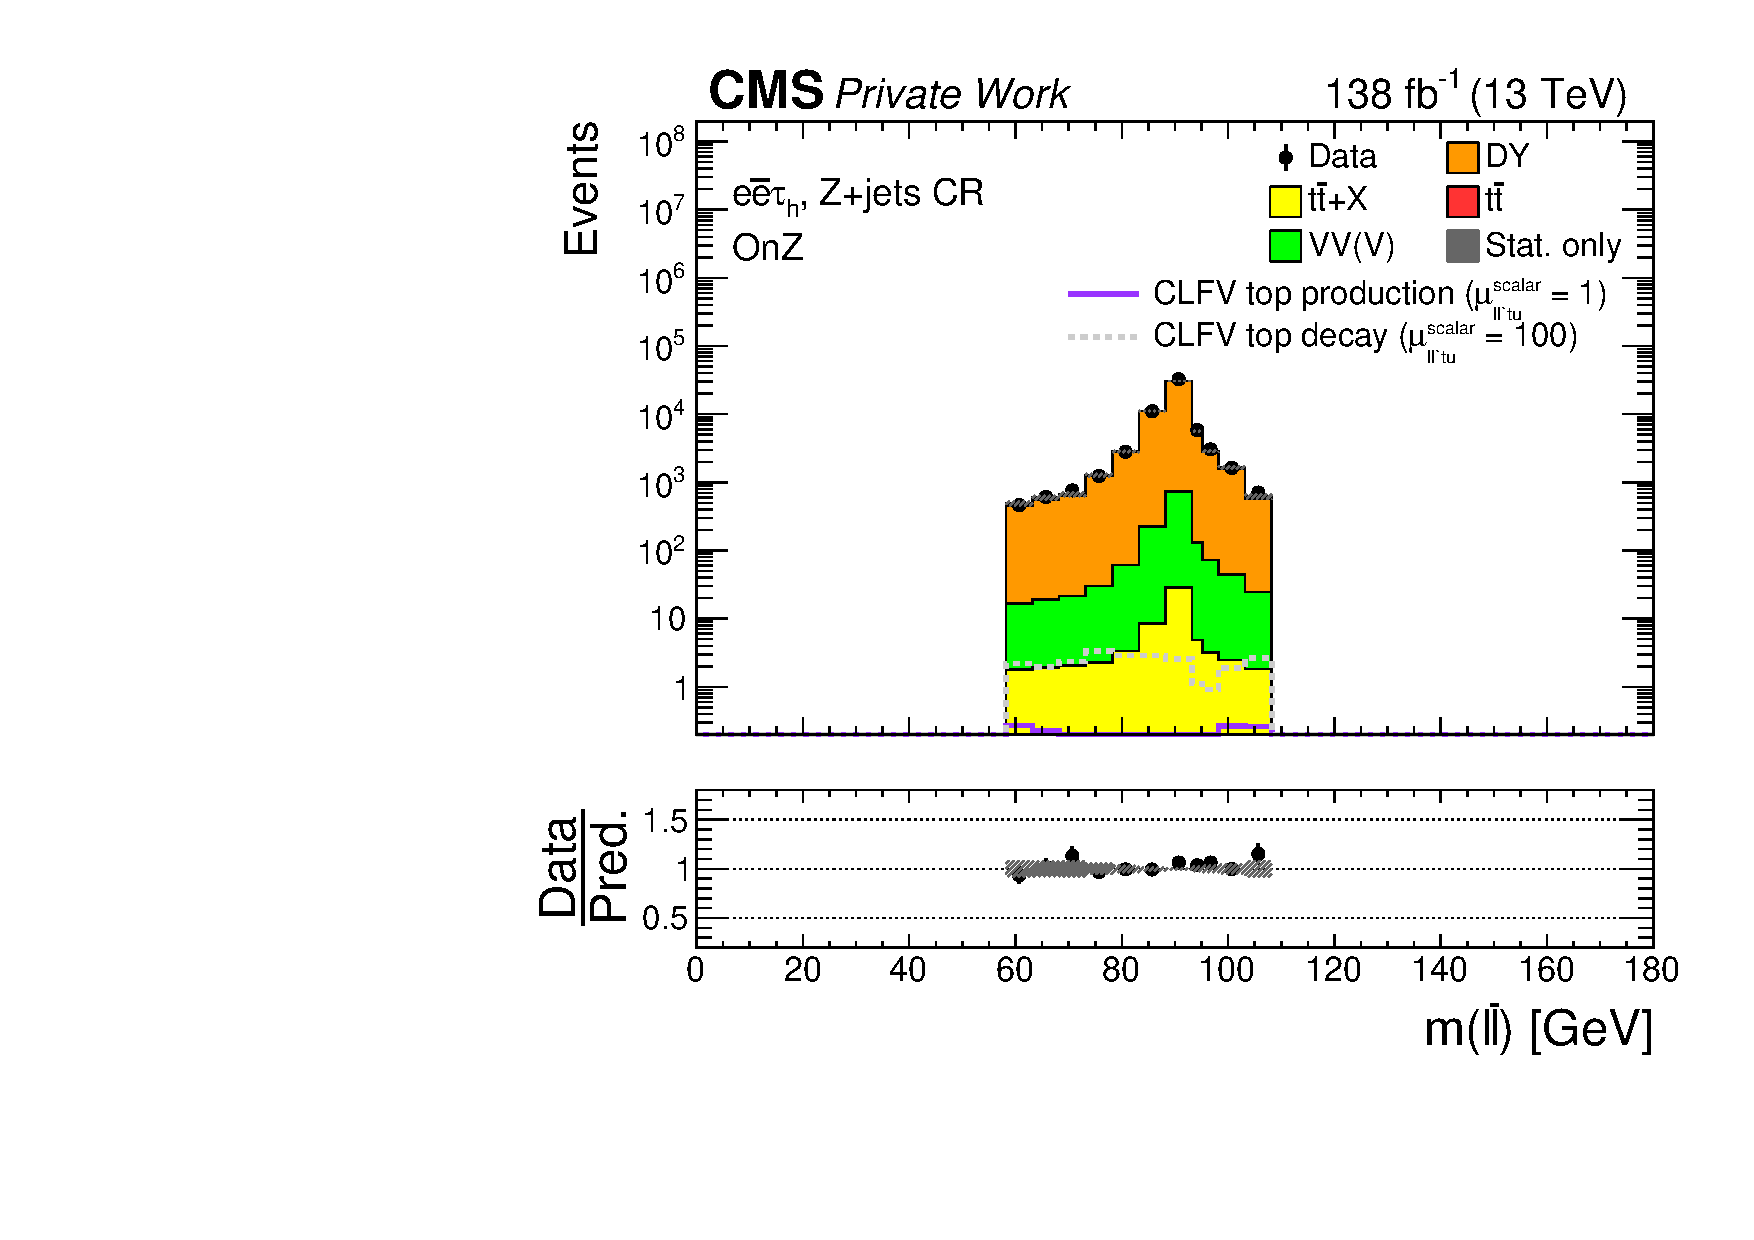
\includegraphics[width=0.48\textwidth]{figures/Part4/Evt/llM_OnZ_ee}&
 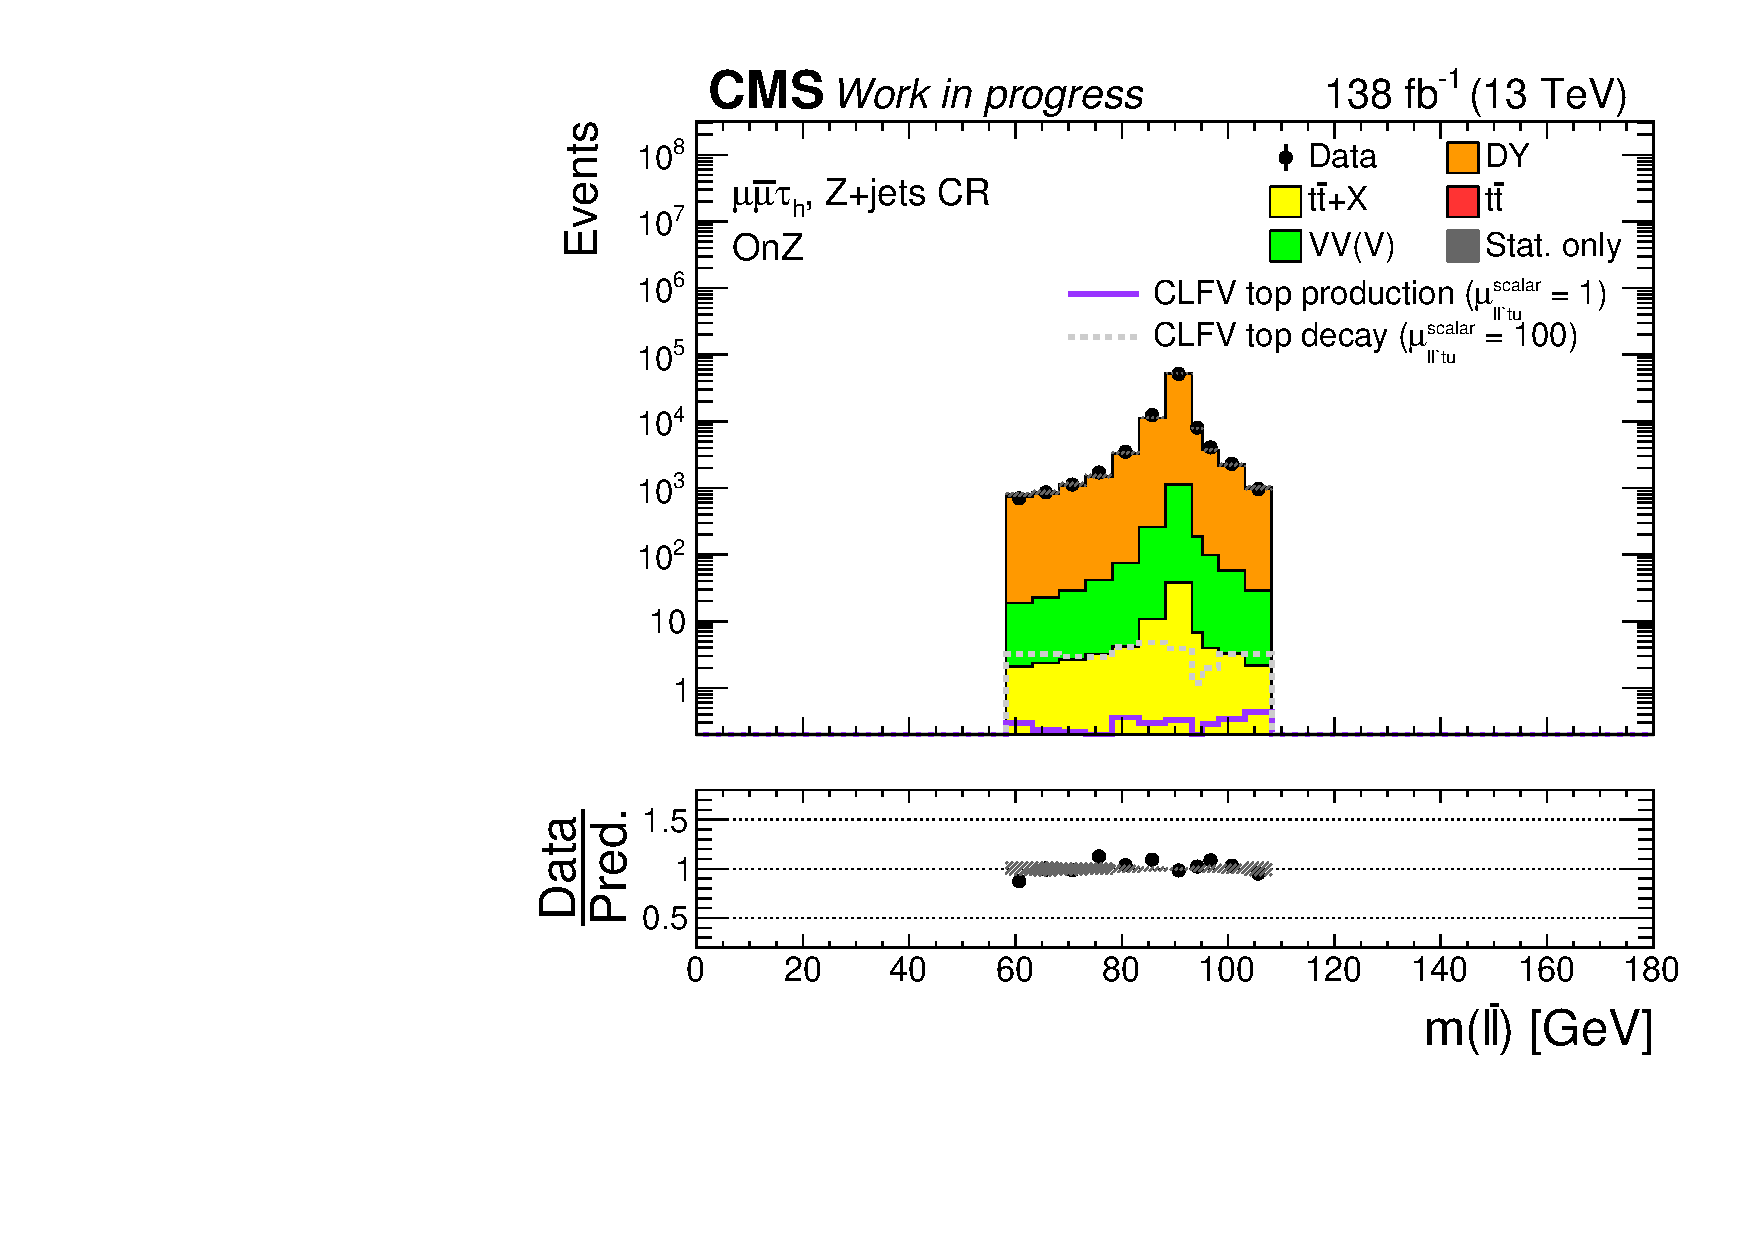
\includegraphics[width=0.48\textwidth]{figures/Part4/Evt/llM_OnZ_mumu}\\
 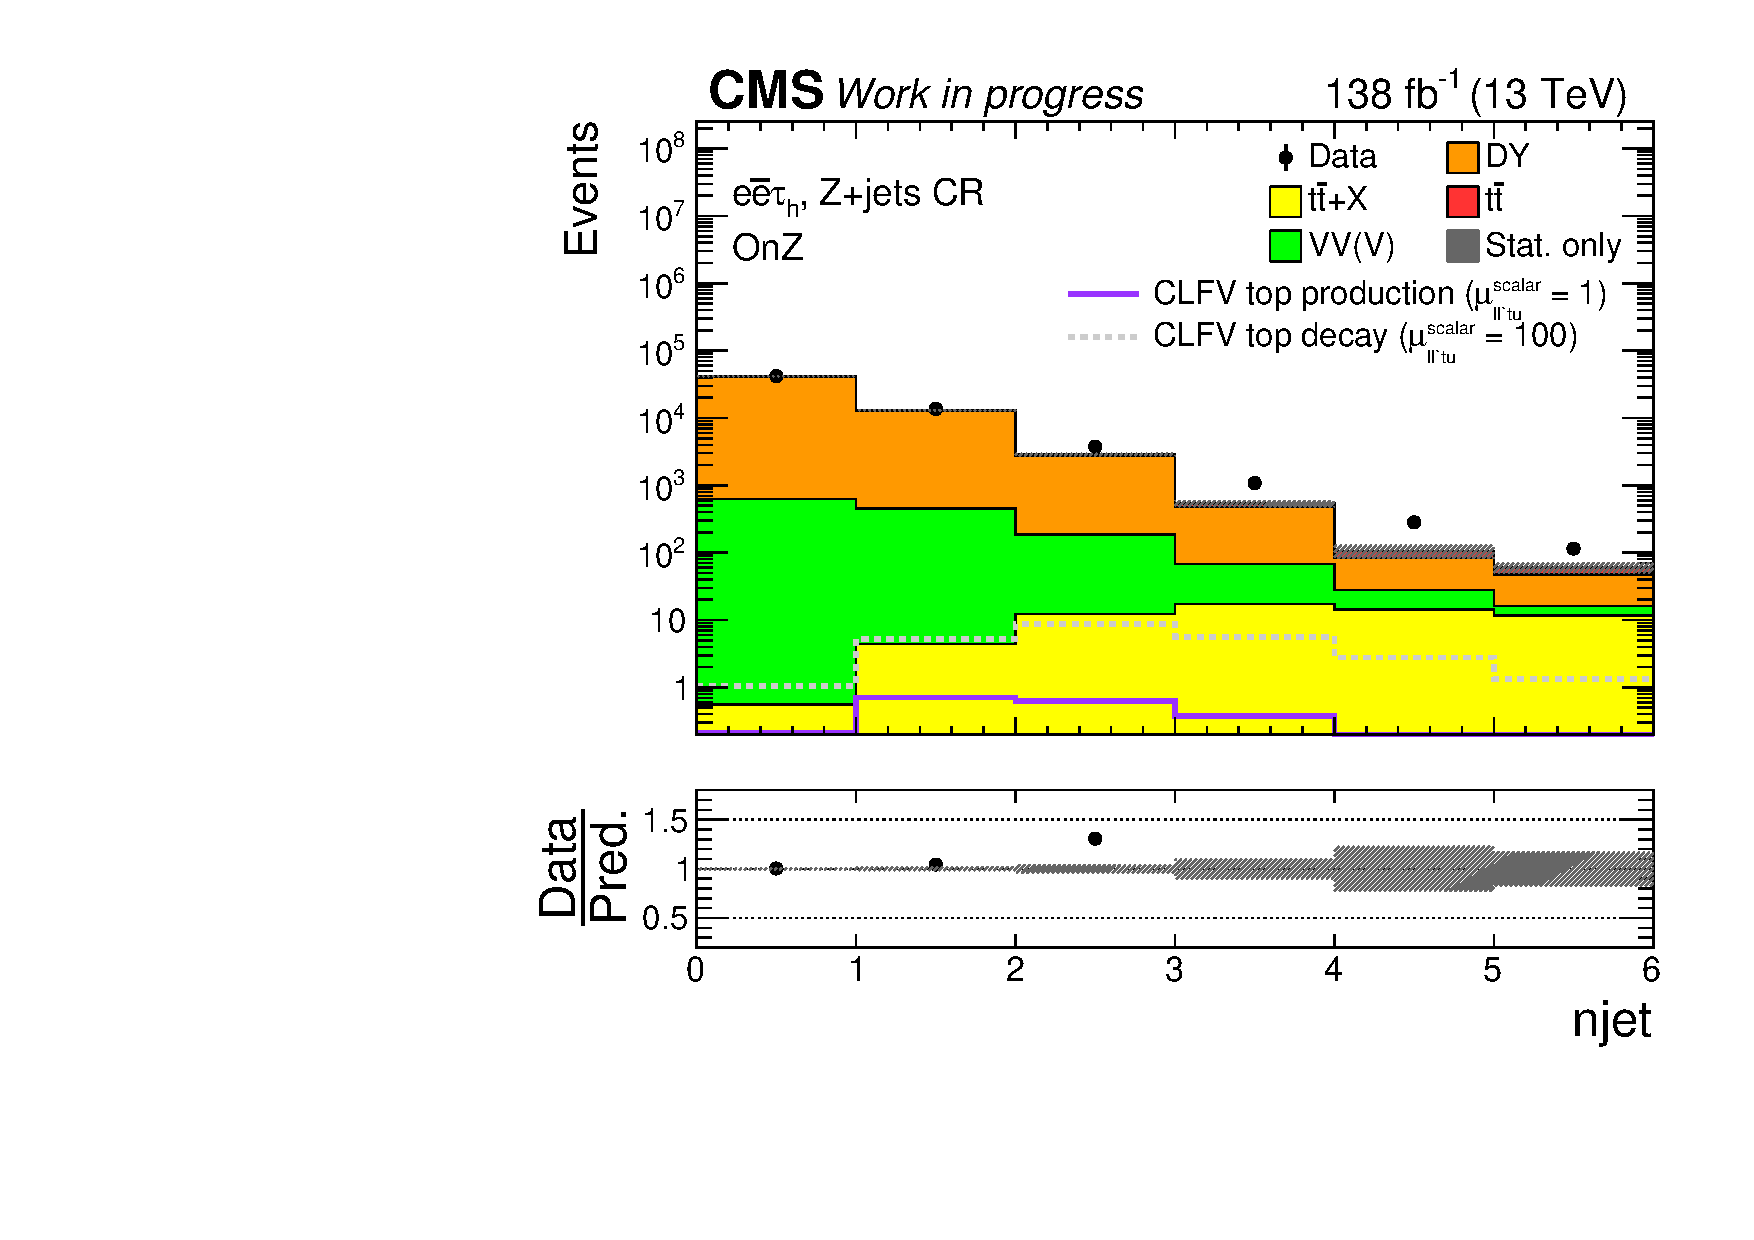
\includegraphics[width=0.48\textwidth]{figures/Part4/Evt/njet_OnZ_ee}&
 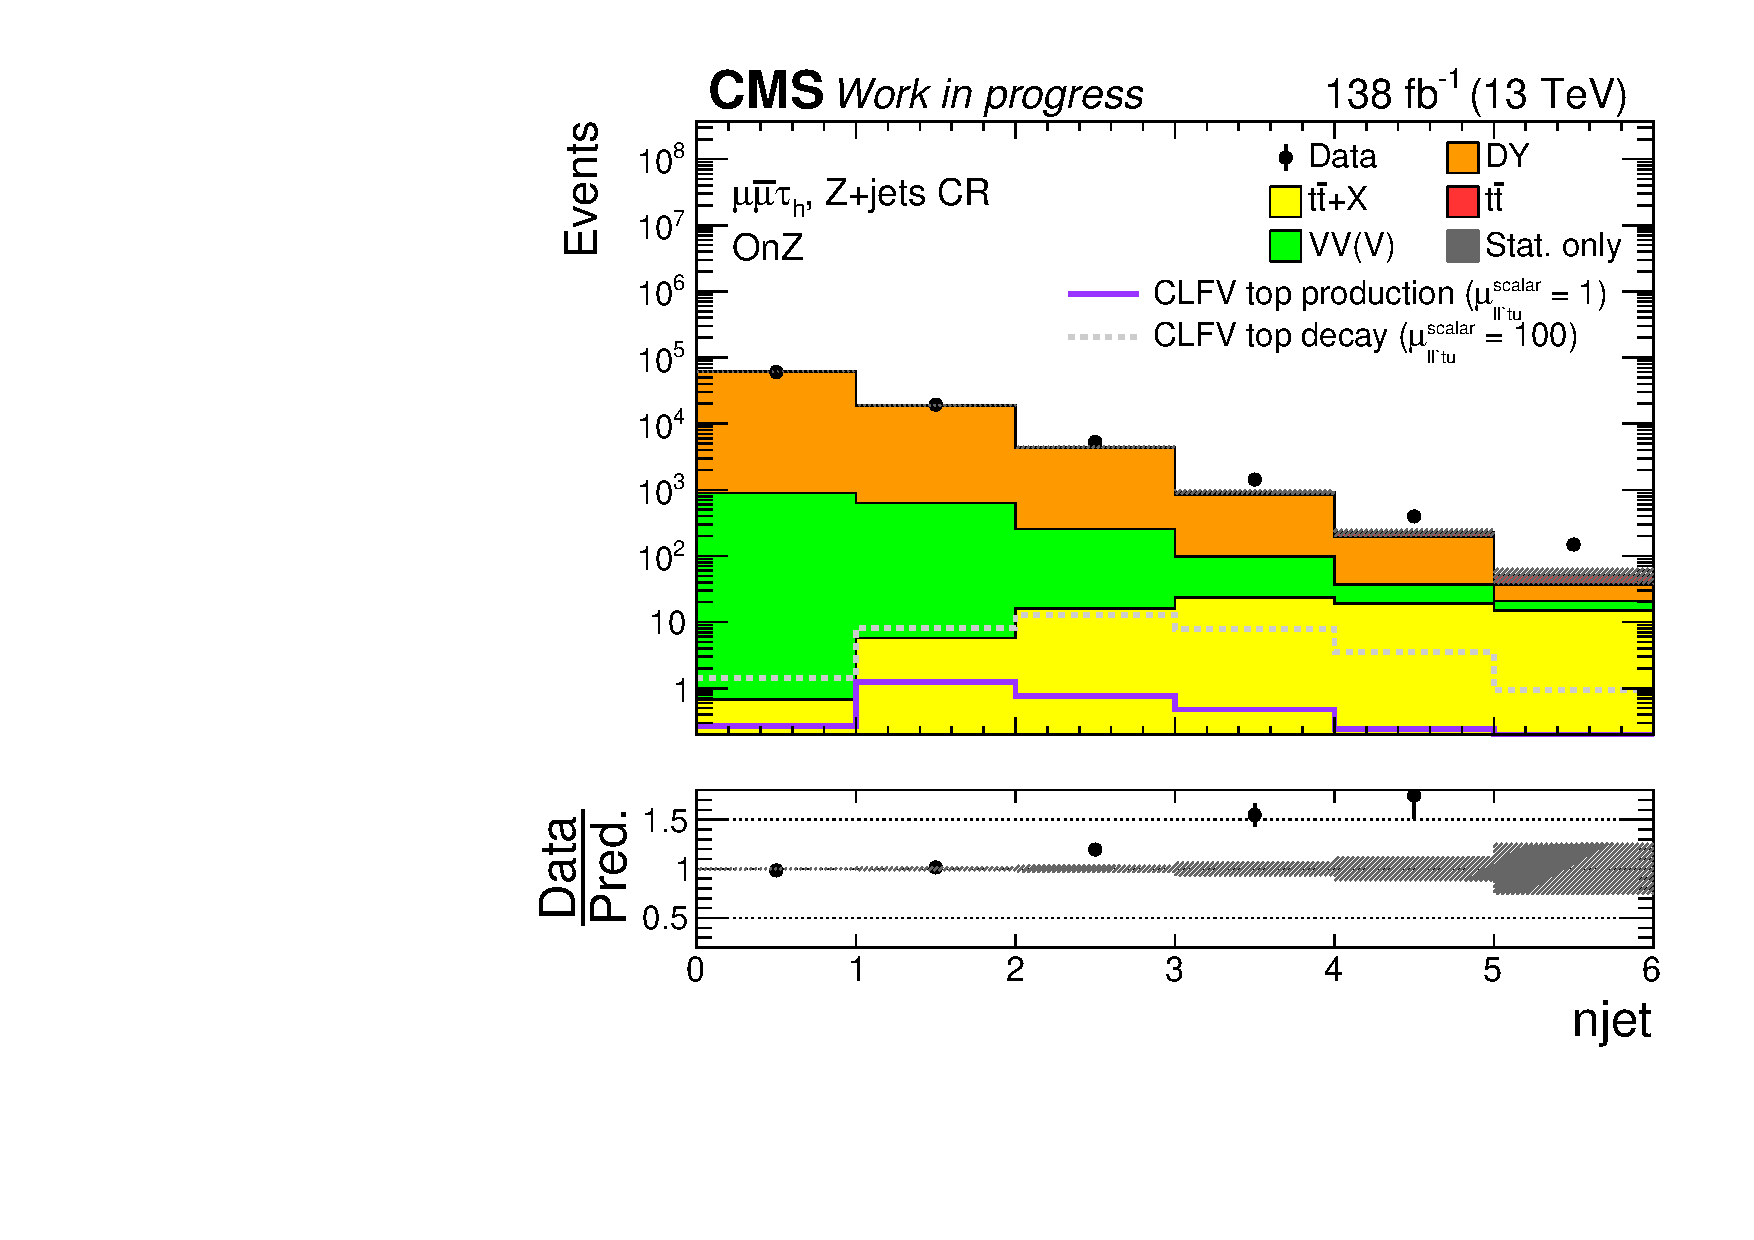
\includegraphics[width=0.48\textwidth]{figures/Part4/Evt/njet_OnZ_mumu}\\
 \end{tabular}
 \caption{Distributions of the \ac{OSSF} lepton mass (top row) and jet multiplicity (bottom row). Events in the \ac{OS}-ee, and \ac{OS}-$\upmu\upmu$ \ac{DY} control regions are shown in the left column and right column, respectively. The data are shown as filled points and the background predictions as histograms. The hatched bands only indicate statistical uncertainties for the background predictions. The last bin of the right column histograms includes the overflow events.}
 \label{fig:DY_CR}
 \end{center}
 \end{figure}